\documentclass[a4paper]{article}
\usepackage[brazil]{babel}
\usepackage{fancyhdr}
\usepackage{graphicx}
\usepackage{amsmath, amssymb}
\usepackage{geometry}
\usepackage{multicol}
\usepackage{enumitem}
\usepackage{float}
\usepackage{titlesec}
\usepackage{setspace}
\usepackage[many]{tcolorbox}
\usepackage{tikz}
\usepackage{keycommand}
\usetikzlibrary{arrows.meta,calc,decorations.pathreplacing}
\geometry{left=1cm,right=1cm,top=0.5cm,bottom=1cm}
\renewcommand{\headrulewidth}{0pt}
\pagestyle{fancy}
\fancyhf{}
\fancyhead[L]{\hspace{5cm}\raisebox{-3cm}{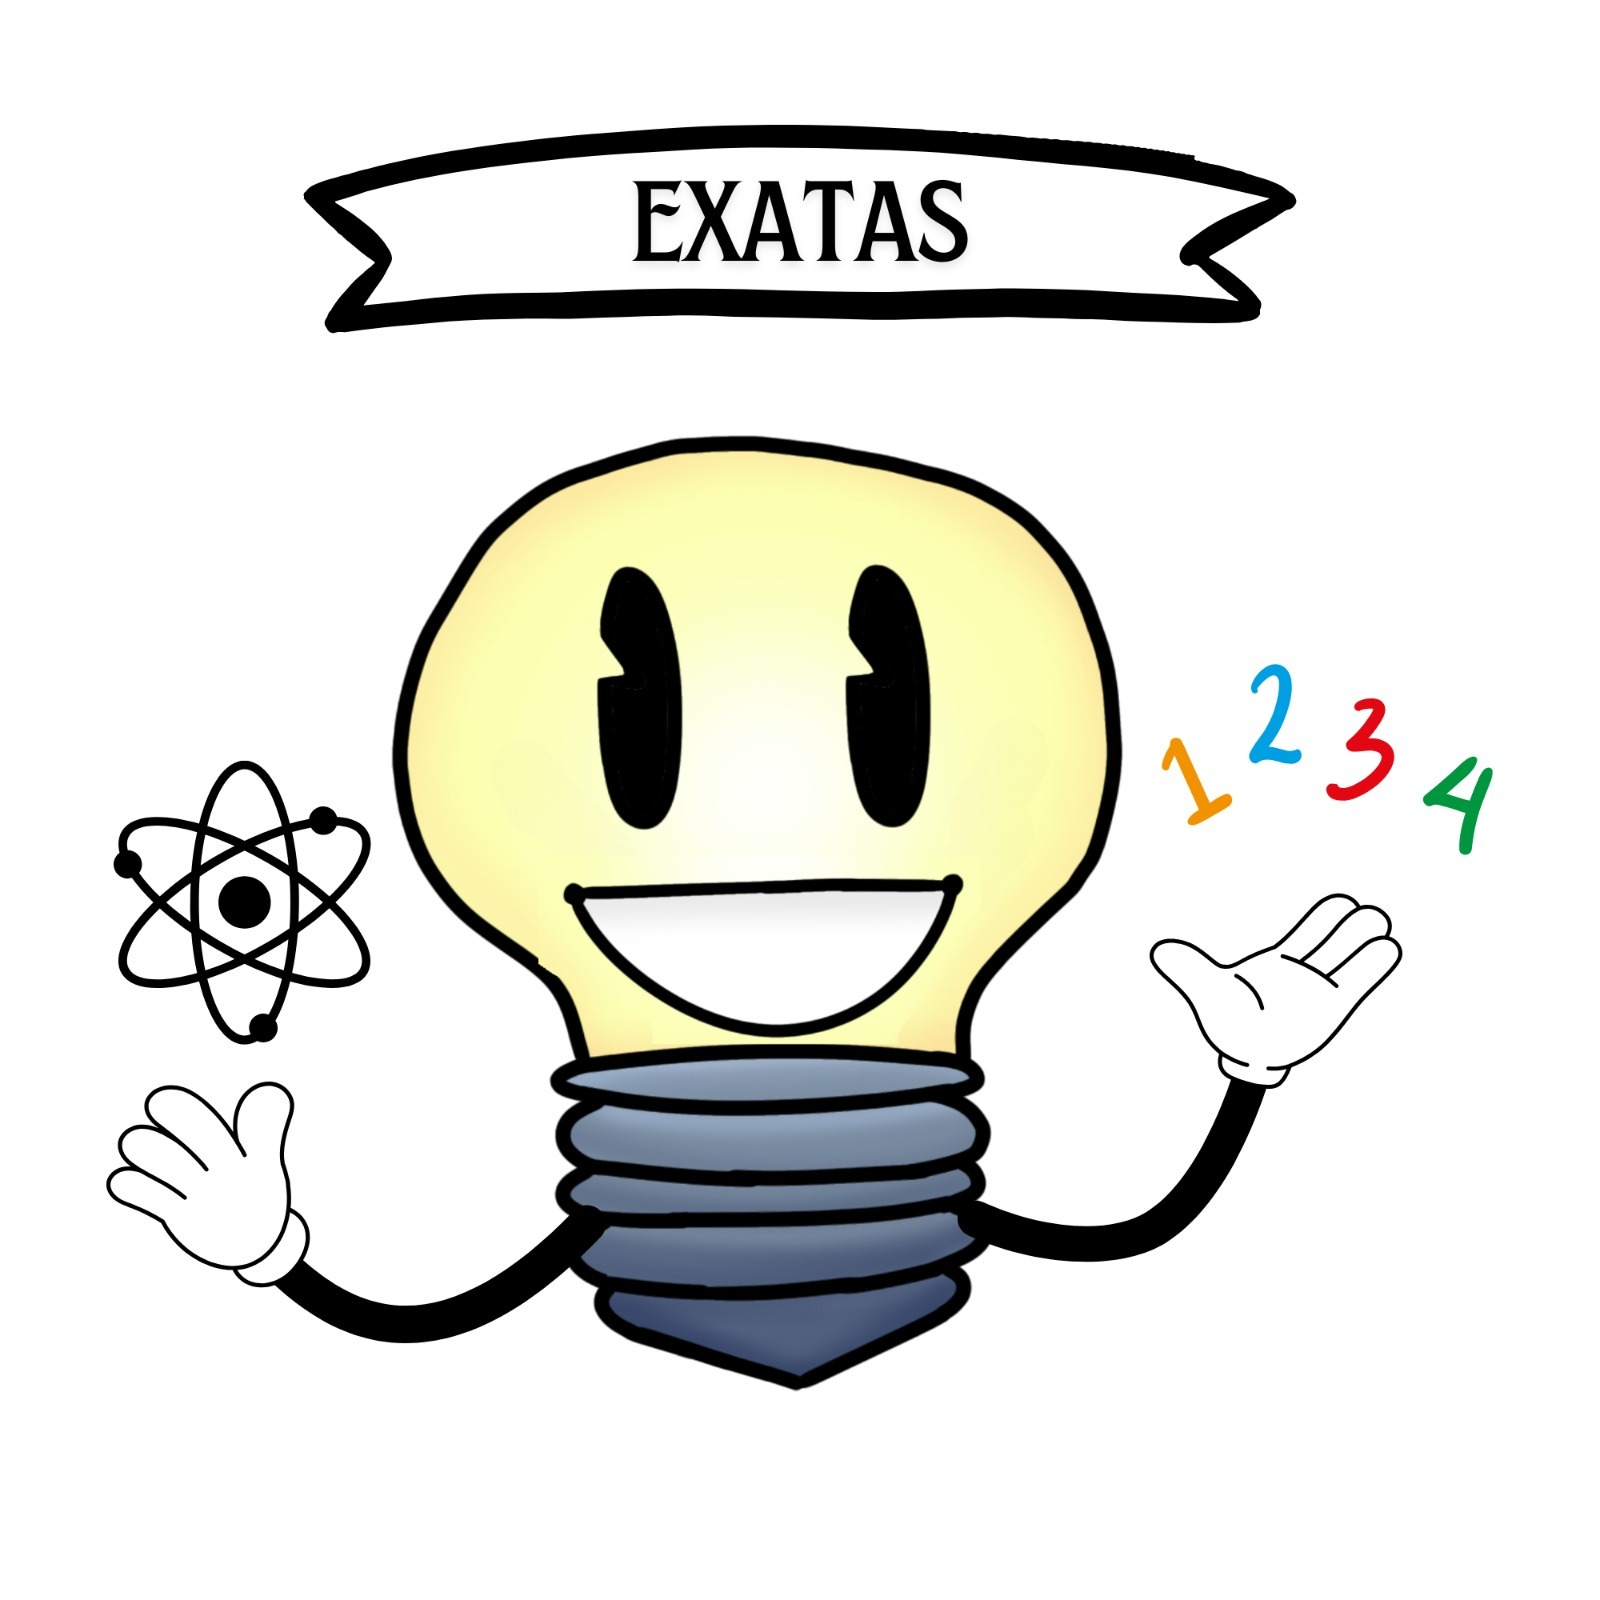
\includegraphics[width=2cm]{exata.jpg}}}
\fancyhead[R]{\hspace{1cm}\raisebox{-2.8cm}{
\includegraphics[width=4cm]{pei.jpg}}}

\begin{document}
	\fontsize{10}{15}\selectfont
	\vspace*{1mm}
	
	\section*{}
	\begin{tcolorbox}[colback=gray!10, colframe=black, boxrule=0.5mm, arc=4pt, title=\textbf{Orientações}]
		A atividade deverá ser entregue até o dia \textbf{30/04}, com todas as resoluções feitas de forma completa e detalhada. Capriche nos cálculos e nas justificativas — isso será valorizado!
	\end{tcolorbox}
	
	\section*{EXPRESSÕES ALGÉBRICAS — RESOLUÇÃO}
	\begin{enumerate}
		\item \textbf{Lucro de Kátia com 45 unidades vendidas:} \\
		Expressão: $L = 8 \cdot u + 4{,}20$ \\
		Substituindo $u = 45$:
		\[
		L = 8 \cdot 45 + 4{,}20 = 360 + 4{,}20 = \boxed{R\$ 364{,}20}
		\]
		
		\item \textbf{Valor do aluguel da máquina:} \\
		Expressão: $L = 280 \cdot D + 10 \cdot Q$ \\
		Substituindo $D = 7$ e $Q = 100$:
		\[
		L = 280 \cdot 7 + 10 \cdot 100 = 1960 + 1000 = \boxed{R\$ 2960{,}00}
		\]
		
		\item \textbf{Média bimestral de Ariel:} \\
		Expressão:
		\[
		M = 0{,}2 \cdot P1 + 0{,}2 \cdot P2 + 0{,}05 \cdot A1 + 0{,}05 \cdot A2 + 0{,}05 \cdot A3 + 0{,}05 \cdot A4 + 0{,}1 \cdot T + 0{,}3 \cdot PF
		\]
		Substituindo os valores:
		\begin{align*}
			M &= 0{,}2 \cdot 3 + 0{,}2 \cdot 6 + 0{,}05 \cdot 8 + 0{,}05 \cdot 7 + 0{,}05 \cdot 5 + 0{,}05 \cdot 9 + 0{,}1 \cdot 7 + 0{,}3 \cdot 8 \\
			&= 0{,}6 + 1{,}2 + 0{,}4 + 0{,}35 + 0{,}25 + 0{,}45 + 0{,}7 + 2{,}4 \\
			&= \boxed{6{,}35}
		\end{align*}
		
		\item \textbf{Substituição de valores na expressão $x^2 + 5x - 8xy$:}
		\begin{multicols}{2}
			\begin{enumerate}[label=\alph*)]
				\item $x = 2$, $y = 2$:
				\[
				E = 2^2 + 5\cdot2 - 8\cdot2\cdot2 = 4 + 10 - 32 = \boxed{-18}
				\]
				\item $x = 5$, $y = -2$:
				\[
				E = 5^2 + 5\cdot5 - 8\cdot5\cdot(-2) = 25 + 25 + 80 = \boxed{130}
				\]
				\item $x = -3$, $y = 4$:
				\[
				E = (-3)^2 + 5\cdot(-3) - 8\cdot(-3)\cdot4 = 9 - 15 + 96 = \boxed{90}
				\]
				\item $x = 2^3 = 8$, $y = 3^2 = 9$:
				\[
				E = 8^2 + 5\cdot8 - 8\cdot8\cdot9 = 64 + 40 - 576 = \boxed{-472}
				\]
			\end{enumerate}
		\end{multicols}
		
		\item \textbf{Cálculo do IMC de Alana:} \\
		Expressão: $\displaystyle IMC = \frac{peso}{altura^2}$ \\
		Substituindo: $peso = 72\,kg$, $altura = 1{,}5\,m$:
		\[
		IMC = \frac{72}{1{,}5^2} = \frac{72}{2{,}25} = \boxed{32{,}0}
		\]
		\textbf{Classificação:} Obesidade Grau I (IMC entre 30,0 e 34,9)
		
		\item \textbf{Área e perímetro da figura:}
		
		Expressões:
		\[
		\text{Área} = \frac{(x + (x+8)) \cdot 6}{2} \qquad \therefore \text{Área} = \frac{(2 \cdot x+8) \cdot 6}{2} \qquad \text{Perímetro} = 6 + x + y + (x+8)
		\]
		
		Substituindo $x = 3$, $y = 10$:
		\[
		\text{Área} = \frac{(2 \cdot 3+8) \cdot 6}{2} = \frac{14 \cdot 6}{2} = \frac{84}{2} = \boxed{42 \text{ unidades}^2}
		\]
		\[
		\text{Perímetro} = 6 + 3 + 10 + (3 + 8) = 6 + 3 + 10 + 11 = \boxed{30 \text{ unidades}}
		\]
	\end{enumerate}
\end{document}
